\section{Introduction}
% Introduction and research questions: What is the problem? Illustrate with an example. What is/are your research questions/contributions? 
\subsection{The Art Gallery Problem}

The Art Gallery Problem \cite{o1987art} is a central problem in computational geometry. It can be introduced as follows: given a simple polygon $P$ with $n$ vertices, we are interested in finding the minimum number of guards (points) that are able to see the whole polygon. A simple polygon is a polygon that has no holes. Thus, we can define the visibility of a point $p$ in the polygon $P \subset \mathbb R^2$. The point (guard) $p \in P$ sees another point $q \in P$ if the line segment $\overline{pq} \subseteq P$. The points that are visible from $p$ form the visibility polygon (region) $Vis(p)$. In the Art Gallery Problem, we are looking for a minimum size guard set $S$ that can see the whole polygon $P$.

Figure \ref{fig:art} displays an example of the Art Gallery Problem \cite{o1987art} with polygon $P$ guarded by 4 points ($|S| = 4$). The visibility region $Vis$ of each guard is marked with a different colour. For point $p \in S$, its visibility region $Vis(p)$ is emphasised with the pink contour. In this case, the vertex $r$ blocks part of the view of $p$ and is called ``reflex'', because the angle it forms on the inside of the polygon is larger than $180^\circ$. Because reflex vertices are only found in concave polygons, convex polygons can be guarded by only one guard.

\begin{figure}[h!]
    \centering
    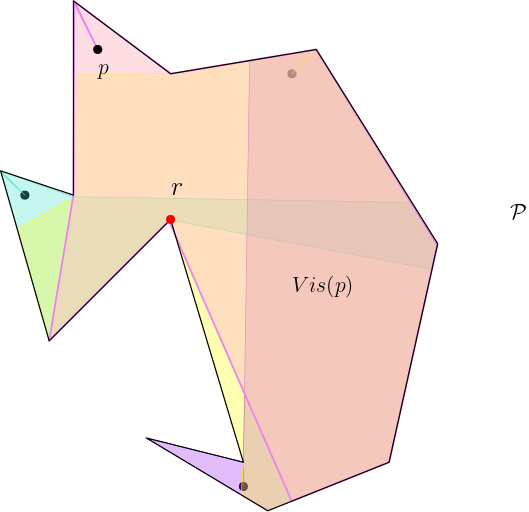
\includegraphics[width = 0.6\textwidth]{p.png}
    \caption{Example of an Art Gallery Problem instance with polygon $P$ guarded by 4 points. The visibility area $Vis(p)$ is emphasised in pink.}
    \label{fig:art}
\end{figure}

The Art Gallery Problem \cite{o1987art} is $\exists \mathbb R$-complete \cite{abrahamsen2021art}, which means it is even harder to solve than NP-complete problems. For this reason, approximation algorithms have been extensively used to address it (\cite{DBLP:journals/corr/BonnetM16b}, \cite{GHOSH2010718}, \cite{DBLP:journals/corr/abs-2007-06920}). Nonetheless, to the best of our knowledge there is no related work on approaching the Art Gallery Problem \cite{o1987art} using gradient descent. As such, we will approach the Art Gallery Problem \cite{o1987art} from a new perspective using gradient descent.

\newpage
\subsection{Gradient Descent}

Gradient descent is an iterative optimisation algorithm for finding the minimum of a continuous differentiable function. The core idea of gradient descent is to repeatedly move in the opposite direction of the gradient of the function at the current point using a specific step size (learning rate). High learning rates result in approaching the optimum faster, but risks overshooting it. Conversely, small learning rates are more precise, with the compromise of a longer computation and convergence time.
When there is no more change in the gradient, then the optimum has been reached. Gradient descent does not guarantee that the found optimum is global. For this reason, it can remain stuck in a local optima.

Figure \ref{fig:gradient_descent} illustrates an intuitive example of applying gradient descent. The optimisation function takes the shape of a curve. Starting from an arbitrary point on the curve, the goal is to reach the minimum of the function (the bottom of the curve). This is done by computing the gradient (derivative) of the function at the current point and moving in its opposite direction. In this case, the gradient would indicate going up the curve. In order to reach the minimum, the point has to move down the curve with the given step size. Continuing from the new point on the curve, the process is repeated until the minimum is reached.

\begin{figure}[h!]
    \centering
    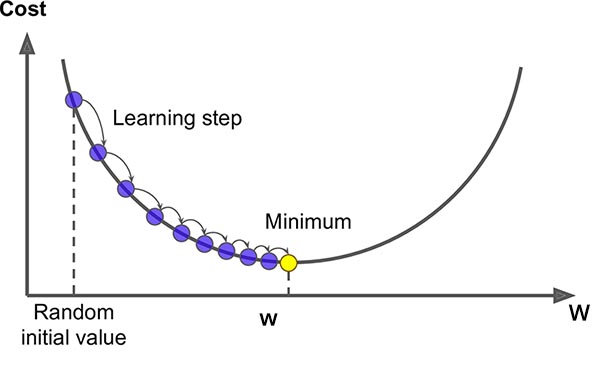
\includegraphics[width = 0.6\textwidth]{external-content.duckduckgo.com.jpeg}
    \caption{Illustrative example of applying gradient descent.}
    \label{fig:gradient_descent}
\end{figure}

\subsection{Thesis Goal}

This thesis will thus be an algorithm engineering paper. The main goal is to create and implement an algorithm that uses gradient descent to approximate the solution to the Art Gallery Problem in reasonably fast time. The algorithm will be implemented in C++ using the CGAL library (\url{https://www.cgal.org}). It will be then compared to other existing algorithm implementations.

As such, preliminary research and implementation is presented as preparation for the thesis project. Section \ref{sec:literature} offers an existing literature overview. Next, Section \ref{sec:theory} describes the relevant theory in detail.
As a preview, Section \ref{sec:experiments} shows some preliminary algorithm implementations and their performance.
Lastly, Section \ref{sec:thesis} presents the development plan for the second phase of the Master's Thesis project.